%\documentclass[conference,compsoc]{IEEEtran}
\documentclass{article}
\usepackage{url,ifthen}
\usepackage[pdftex]{graphicx}
\title{What does it mean to own our genes?\\
{\small Genetic De-anonymization Attacks and Implications for Privacy}}
%Draft}}
\author{Arvind Narayanan \\
{\small Stanford University}}

\newcommand{\XX}{{\cal X}}
\newcommand{\YY}{{\cal Y}}
\newcommand{\Adv}{\textsf{Adv}}
\newcommand{\PP}{\textsf {PP}}
\newcommand{\PR}{\textsf {PR}}
\newcommand{\bkg}{\textsf {BkGnd}}
\newcommand{\priv}{\textsf {priv}}
\newcommand{\pub}{\textsf {pub}}
\newcommand{\Aux}{\textsf {Aux}}
\newtheorem{definition}{Definition}

\newcommand{\grumbler}[2]{\begin{quote}\sl{\bf #1:} #2\end{quote}}
\newcommand{\arvind}[1]{\grumbler{Arvind}{#1}}

\newcommand{\ie}{\textit{i.e.}}
\newcommand{\eg}{\textit{e.g.}}

\begin{document}
\maketitle




\begin{abstract}
Given that each of us shares genetic material with our blood relatives, to what extent can one expect to keep one's genetic information private? We consider this question with respect to an attacker equipped with large-scale (albeit incomplete and ``noisy'') information about the blood relationships in a large population group. 

Given this kind of auxiliary information, it turns out that the availability of genotype information of a small fraction of individuals -- as little as 0.1\% -- is enough to cause the majority of the population to lose any hope of genetic privacy. We develop a strong inference attack that allows the attacker to re-identify completely anonymous genetic material, such as pieces of hair collected {\em en masse} from public spaces without the consent or even the {\em knowledge} of the potential victims.

We survey the efforts aimed at aggregating genealogical  data on a massive scale and argue that the compilation of the ``world's family tree'' is a matter of time. Further, we point out several population groups for which enough auxiliary data is {\em already} available to leave them vulnerable to genetic re-identification.

There is no purely technological fix to our attack. We briefly present policy prescriptions that may delay ubiquitous genetic re-identifiability, and argue that genetic privacy norms must change to accomodate the new technological reality. In particular, the notion of an ``owner'' of each piece of genetic data appears no longer tenable.
 
%The right of a person to control his or her own data is a fundamental tenet of privacy advocacy today. This position implicitly assumes the {\em possibility} of such control, at least with the co-operation of the powers that be -- broadly, the government, and those involved in data collection and analysis. Our attack shows that the notion of an ``owner'' of each piece of data may need to be jettisoned entirely, necessitating an overhaul of the genetic privacy debate.

%In the context of genetic data, it is well known that each person shares genetic material with blood relatives, and that the extent of sharing is dependent upon the degree of the relationship. Given this fact, how does the notion of an ``owner'' of each piece of data hold up? Does it merely need to be modified, or jettisoned entirely, thus necessitating an overhaul of the genetic privacy debate?

%We show that the answer is likely to be disturbingly close to the latter possibility. The key to our conclusion is an analysis of what an adversary, equipped with realistic ``auxiliary information,'' might be able to deduce from completely anonymous genetic material -- for instance, pieces of hair collected {\em en masse} from public spaces without the consent, or even the {\em knowledge}, of the potential victims. We qualify and quantify the conditions under which identities can be affixed to these surreptitiously collected samples, and argue that these conditions will become a reality within a few short years.

%There does not appear to be a purely technological fix to our attack. We briefly present policy prescriptions that may delay the eventuality of genetic re-identifiability, and argue that genetic privacy norms must change to accomodate the new technological reality.
\end{abstract}

\section{Introduction}

Threats to genetic privacy have been of concern to society since the proliferation of DNA profiling a few decades ago. However, the availability of cheap genotyping in the last few years has changed the scale of the threat so greatly as to make it qualitatively different. At the time of this writing, a ``personal genomics'' kit costs \$399 \cite{23andme-store} and has been estimated to capture over 50\% of the entropy in the human genome \cite{snpentropy}.

Privacy violations could take many forms such as data breaches and non-consensual information sharing. Protection against such violations falls under the domain of public policy, law enforcement and computer security. We are instead concerned about {\em inference attacks}, which result in unexpected revelation of sensitive facts about individuals from genotype data or DNA samples that might at first glance appear to hide the facts in question.

Inference attacks have recently received considerable attention: in 2007, Homer {\em et al} showed how to determine  if an individual contributed DNA to a mixture, by analyzing only the {\em aggregate} values of each genotype locus. Further papers have discussed this attack, arguing that it is either less serious \cite{sriram} or more serious \cite{gwa-privacy} than previously thought.  In other work, Goodrich analyzed threats to the privacy of mitochondrial DNA sequences \cite{mastermind}.

Common to these attacks is the fact that the victim needs to have first voluntarily provided an identifiable DNA sample. On the other hand, we consider the question of what an adversary can learn from a completely anonymous genetic sample -- for instance, pieces of hair collected {\em en masse} from public spaces without the consent, or even the {\em knowledge}, of the potential victims.

Our analysis rests on the asssumption that two types of data will soon become available to powerful attackers (Sections \ref{genealogy-survey} and \ref{genotype-survey} are dedicated to justifying and quantifying these claims):
\begin{itemize}
\item
A {\em genealogical graph} representing of a significant fraction of all blood relationships among a large population group.
\item
{\em Genotypes} of a small fraction of the individuals represented in the above graph.
\end{itemize}

Blood-related individuals share fragments of their genome; such shared genetic sequences, known as ``identical-by-descent'', or IBD, exist with significant probability for pairs of people related by as little as a single common ancestor 5--7 generations ago. Furthermore, fast algorithms to identify identical-by-descent segments between have recently been developed \cite{germline}. This enables an adversary to (probabilistically) detect even remote blood relationships among individuals.

Our main technical contribution is an inference attack that uses IBD segment detection to infer the identity of an unlabeled genotype. The attacker's input is a 1) genealogical graph, 2) a set of labeled genotypes, the labels being nodes in the graph, and 3) an unlabled genotype. First, the attacker computes IBD segments between the unlabeled genotype and each labeled genotype, using existing algorithms. He then uses these sets of IBD segments to determine the node in the graph that is most likely to correspond to the unlabeled genotype, using a novel algorithm.

We say that our attacks succeeds if it identifies the correct node\footnote{This is a slight oversimplification: in reality, the algorithm outputs a ``sibling group,'' since siblings of the same sex are indistinguisable from genotypes alone.}, or if it correctly deduces that genotype did not come from any individual represented in the graph. The attack has several strengths:
\begin{itemize}
\item
It requires only a small fraction of labeled nodes to succeed -- in our experiements, as little as a tenth of a percent in some cases (see below). 
\item
It can tolerate ``noise'' in the form of missing as well as incorrect links in the graph. This is vital: while increasingly massive genealogical graphs are becoming available (Section \ref{genealogy-survey}), these are by no means complete nor fully accurate.
\item
It makes no assumptions about the nature of mating -- i.e, monogamy vs. polygamy, inbreeding coefficient, population growth rate, mixing model (random vs. geographically or socially structured), etc. While these differences do affect the efficacy of the attack somewhat, the algorithm remains the same in all cases.
\end{itemize}

Let us walk through a simple example to illustrate how the attack might work. Let us call our victim Victor, the individual whose genetic information the adversary possesses.  Victor's node happens to be somewhere in the genealogical graph available to the adversary; the adversary, not yet knowing this, would like to find out if that is in fact the case, and if so, determine the identity of the node. Suppose that two of Victor's cousins Peggy and Sue have labeled genotypes available in the graph. Furthermore, assume that Victor is related to Peggy through his mother and to Sue through his father.  

\begin{figure}[htp]
\begin{center}
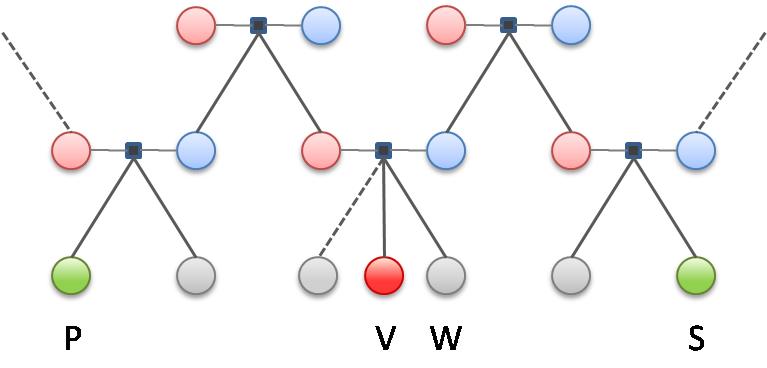
\includegraphics[height=2in]{attack-illustration.png}
\end{center}
\caption{Illustration of attack}
\small{
The red node represents the victim. 
The green nodes represent individuals whose genotypes are available to the attacker.
Pink and blue nodes represent females and males respectively.
The thick lines represent genealogical links that are available to the attacker, and the dotted lines represent links that are not available.}
\end{figure}

Given this setup, the adversary can now determine that unlabeled genotype comes from someone who shares 1/8 of their DNA with both Peggy and Sue.\footnote{The attacker can deduce more than this: for instance, analyzing the {\em number} of shared segments in addition to their {\em total length} can tell him that the related individuals share a pair of grandparents, rather than one being a great-grandparent of the other, which would also result in a $\frac{1}{8}$ shared genome. However, we ignore this for the purpose of this  example.} Intuitively, if all mating pairs in the family tree are a) monogamous and b) have no recent common ancestor, then the only nodes that satisfy the constraints available to the adversary are Victor, and any siblings he might have. The adversary looks at the graph and determines that the sample came either from Victor, his brother Wilbur, or any other siblings he might have who are not represented in the graph.

Since it is impossible to distinguish between siblings without further auxiliary information, our algorithm outputs the most likely ``sibling group'' instead of the most likely individual. We consider the attacker to be successful if the sibling group is guessed correctly. In Section \ref{genotypephenotype}, we outline how to carry out further de-anonymization using other auxiliary information. Thus, even if Victor has not been completely de-anonymized, it can serve as useful starting point for manual analysis which can complete the de-anonymization.

Unlike our toy example above, in reality the inference is far more complex. The primary difficulty arises due to the fact that only small fraction of labeled genotypes available to the attacker.  With 0.1\% node-genotypes available, for a random unlabeled node we can expect that not a single one of its 4th cousins (or any closer relative) is among the genotyped set.  At low levels of genetic sharing, it becomes impossible to determine the exact familial relationship, and complex statistical calculations are necessary.

Furthermore, in our example we assumed monogamy, a lack of inbreeding, and an absence of errors; overcoming these assumptions also presents a great challenge.

We now summarize our quantitative results. {\em [numbers go here]}.

The rest of the paper is organized as follows. In Section \ref{genealogy-survey}, we survey techniques and projects aimed at compiling genalogical graphs of large populations. The scale and ease of data availability may surprise the reader. In section \ref{genotype-survey}, we discuss genotype databases and how an attacker may obtain them. We also point out population groups that are most immediately at risk from our attack.

 In Section \ref{reidentification}, we present a survey of re-identification techniques in computer science and their implications for data privacy. Having been virtually unknown to privacy analysts merely a decade ago, advances re-identification science has now thrown into question the very notion of anonymized data.

Section \ref{genetics-background} is a very brief recap of the genetics required to understand our attack, in particular the manipulation of genetic information that occurs during meiosis. We also describe the ``GERMLINE'' IBD-detection algorithm of \cite{germline}, and motivate a few simplyfing assumptions that we make in our model.

Section \ref{attack} describes our attack methodology and algorithm in detail, and Section \ref{results} contains the results of our experiments. We conclude by discussing the implications of our attack to society in Section \ref{discussion}.


%\section{Data collection survey}




\section{Genealogical Databases: A Survey}
\label{genealogy-survey}
Recall that there are two types of data that are crucial to the success of our attack: genealogical data and  genotypes of known individuals. This section concerns the former; we survey a) the types of original data sources that can be used to compile genealogical graphs and b) the existing organizations and databases of genealogical information. 
In the interest of brevity, we focus on the U.S. and the U.K.; information about other countries is summarized in Appendix [].

First, let us consider the process of constructing a genealogical graph from one or more databases of individual records, where there are no links present either between records or between the different databases.  There are three main algorithms that are needed:

{\bf Entity resolution}, also known as identity resolution, and in the genealogy context as record matching or record linking. It involves resolving records across different databases as the same entity, based on a fuzzy matching of attributes; a simple example would be matching names via Soundex. Record linkage is an extremely well-studied problem and as one might imagine, has applications everywhere. W.E. Winkler of the U.S. Census Bureau has authored two surveys \cite{winkler-survey-99,winkler-survey-06} from the statistics perspective.

{\bf Lineage linking} refers to the inference of (kin) relationships between individuals, and the techniques used are similar to record linking. For example, using the parents' names reported in a birth record to link an individual to the resolved entities corresponding to the parents constitutes lineage linking. A lineage-linked database of individuals is essentially a genealogical graph, albeit possibly containing errors and inconstencies.

GEDCOM is a widely used standard for lineage-linked data developed by the LDS Church; an example GEDCOM record can be found in \cite{wp-GEDCOM}.

{\bf Graph merging} operates at a more global level, and tries to merge two genealogical graphs. As opposed to record linkage, graph merging algorithms are still in their infancy, and little information exists in the published literature. 
The first mention of graph merging was by Wilson \cite{wilson-merging}. Sweet {\em et al.} provide a semi-coherent account of a different algorithm \cite{enhanced-merging}.

Agarwala {\em et al.} \cite{anabaptist} describe merging two genealogies of the North American Anabaptist population consisting of around 56,000 and 31,000 individuals respectively. Interestingly, new relationships are created in the merged graph which do not exist in either original graph. 


%Merging is employed by the LDS in creating the ancestry file.  

{\bf Living vs. deceased persons.} Recall that although the privacy harms of our attack (or any other attack) impact only the living, our modus operandi is to find remote familial relationships between individuals via distant common ancestors (5-7 generations). This means that it is important for the attacker to have auxiliary information in the form of genealogical data extending back well into the nineteenth century.

Obtaining data on deceased persons turns out to be significantly different from living persons. There are two key differences: many sources of genealogical data apply (some) privacy controls for living persons, and usually none for deceased persons. Second, data on deceased pesons has often been irretrievably lost, especially the farther one goes back in time, whereas for living persons the information exists at least in human memory, even if it may not be easy for the attacker to obtain.

%In the light of the different level of availability for records pertaining to living and dead people, not only from official bureaus but also from private organizations such as the LDS church (see below), we divide our survey into these two categories.

Let us now turn to data sources. Broadly, these can be divided into official sources and user-contributed data. Official sources further subdivide into vital records, census records, and other miscellaneous public sources such as voter registration lists and property records.

\subsection{Vital records}

Birth, death, marriage  and divorce records are collectively known as ``vital records.'' In the United States, vital records are typically maintained at the state level. These records are for the most part public, although not always available {\em en masse} in digital form. A summary of availability can be found in \cite{messing}. Some salient points to note are:
\begin{itemize}
\item
Birth records are ``aged'' by between 50 to 75 years, i.e., some information is redacted in records that are less than that age.
\item
Each county maintains records in microfiche form, but most of the larger states aggregate this information in digital form at the state level. 
\item
The authors note that ``as time progresses, public information stored at even the smallest county offices will invariably become digitally available."
\end{itemize}

In the United States, there is a drop-off in the availability of vital records before the 1900s. The situation in European countries is much better: In the United Kingdom, for instance, vital records have been collected since at least 1837 \cite{ukbmd.org.uk}. Data from prior dates is often available from parish registers from individual counties.\footnote{Need survey of more European countries.} 

Vital records may be made available by official bureaus either in original paper form, or in microform, or electronically. The process of converting from paper to an indexed electronic database involves two steps:

{\bf Digitization} First, the paper records are converted into microfilm or microfiche. These are document storage formats that physically compress the size by a factor of 25 or more \cite{wp-microform}. The microform documents are then converted to digital images using a microfilm/microfiche reader. 

{\bf Transcription} Next, the resulting images are converted into text. Many organizations involved in making vital records available online achieve this time-consuming step by ``crowdsourcing'' it to volunteers participating over the Internet.

Constructing a genealogy from vital records is not trivial, but can in large part be automated: 
\begin{itemize}
\item
The information available -- first and last name, place (to the resolution of a county), and age -- is usually sufficient to carry out record linking, even in the absence of unique identifiers.
\item
For unredacted or ``aged'' records, the parents' names are available. Combined with other attributes, this makes lineage linking possible.
\item
Even when the parents' names have been redacted, Griffith and Jakobsson \cite{messing} provide a variety of heuristics that they use to infer the mother's maiden name; many of these heuristics can also be used for lineage linking.
\end{itemize}

\subsection{Census records}

Census records are an invaluable source of genealogical research. In the United States, they are maintained by the National Archives \cite{nara-census}. The first Federal Population Census was taken in 1790, and has been taken every ten years since. Due to privacy reasons, data is available only for the 1930 and earlier censuses. The National Archives makes census records available on microfilm from 1790 to 1930. These have been completely transcribed by private companies, and partially by non-profit organizations (see below).

The following information is available for each individual covered by the 1850-1930 censuses: name, age, state or country of birth, parents' birthplaces, year of immigration, street address, marriage status, years of marriage, occupation, and a few other attributes. The situation in the UK is similar in terms of information available; micro-data from the 1851-1901 censuses are currently public.

Record linkage across censuses is possible, and there are a number of efforts to unify the micro-data across the historical censuses; for instance, see \cite{ipums-usa}. Lineage linking is possible to an extent because the members of a household are listed together; however, census records alone provide no definite link between a woman's maiden and married names. We are not aware of any efforts to derive lineages from census records, but they may serve as an excellent complement to vital records.


\subsection{Other public records}

The National Archives website claims that federal records are a ``treasure chest of genealogical information'' \cite{nara-faq}. Military, immigration, naturalization and land records are some other types of official records that are useful as genealogical sources. 
More information can be found in \cite{nara-faq}. 

Land and property records from earlier periods can be particularly useful because deeds contain very detailed information in an effort to identify the individual as completely as possible. Modern property records can be useful for tracking people who move to a different state \cite{messing}; they may have more uses for genealogy since a person's relatives are often identified in these records. 

Voter registration records in the United States have been public since 1995 by the National Voter Act of 1993. They are particularly useful for genealogical reconstruction because they provide a connection between married and maiden names \cite{messing}.

The Social Security Death Index -- which was created as a way to prevent identity theft of the recently deceased -- can used in enabling privacy breaches, as recently demonstrated by Acquisti and Gross \cite{acquisti-ssn}. According to Griffith and Jakobsson, the SSDI improves the ability to link death and marriage records \cite{messing}.

\subsection{Secondary sources of official records}

As noted above, official records are often made available only in microfilm, and may not be available from a central source. Even after digitization, there remains the task of constructing a lineage-linked database, and of aggregating different databases. The availability of such cleansed and aggregated data makes a huge difference to the practical feasibility of our attack. Considering that the source data is public, it is quite likely that the processed data will eventually become publicly available. Nevertheless, it is important to survey the current availability of official records from secondary sources.

{\bf Ancestry.com}, Inc., based on Provo, Utah, is the largest for-profit genealogy company in the world \cite{wp-ancestry.com}. It operates a variety of subscription-based websites including ancestry.com, genealogy.com, myfamily.com and rootsweb.com. The company scans and indexes essentially every category of official record of relevance to genealogy \cite{ancestry.com-cardcatalog}. In particular, they have a complete the index of all U.S. Census lists for which micro-data is available, and all U.K. census micro-data starting with the 1841 census. Their indices of U.S. vital records is also nearly complete. 

Ancestry.com claim to have indexed over 4 billion records; however, it must be borne in mind that the number of distinct individuals covered by these records is likely to be much smaller. They also claim to perform lineage-linking; see details in Section \ref{genealogy-user}.

{\bf FreeBMD} is a UK-based charitable organization that has the goal of creating a free transcription of vital records (called ``BMD," for ``Births, Marriages and Deaths'' in the UK context), and making them freely available online for search or download.  The index is nearly complete; currently, over 170 million unique records have been transcribed \cite{freebmd}.

{\bf FamilySearch} is a project of the U.S.-based {\bf Church of the  Latter Day Saints.} The LDS church maintains the International Genealogical Index, which comprises both user-contributed records and records transcribed from official sources. There are currently 200 cameras converting vital records into microfilm, and the transcription process is crowdsourced. Recently, the number of transcribed reached 250 million \cite{familysearch-250m,familysearch-indexing}. This data can be searched online without a fee.

Several companies such as Choicepoint and Intelius aggregate property records (as well as a number of other types of public records such as tax and court records). We are not aware of any efforts at such aggregation by non-profit entities.\footnote{this paragraph needs expansion.}

\subsection{User-contributed genealogy}
\label{genealogy-user}
User contributed genealogy is looked down upon by professional genealogists as error-prone. From the computer scientist's perspective, however, more data is almost always better; sophisticated algorithms can help filter out noise correct inconsistent information. Besides, the accuracy requirements of genealogical data for our attack are much lower than for traditional applications of such data.

Ancestry.com claims 400 million names in user-contributed family trees \cite{ancestry.com-worldtree}. It is not clear if this number represents de-duplicated records. Another service offered is ``{\bf OneWorldTree},'' which integrates user-contributed data with official records \cite{ancestry.com-oneworldtree}. They claim to perform ``stitching'' of family trees as part of OneWorldTree, which we interpret as graph merging. The size of the merged graph is not stated. As with all ancestry.com services, a subscription service is required for online (search-only) access to these graphs.

The LDS Church maintains the {\bf Ancestral File}, which is a user-contributed, lineage-linked database of 35 million names \cite{familysearch-ancestralfile}. The size of the largest connected component is not clear. It is available to search online without a fee. An API is available with a license for software affiliated with the Church \cite{familysearch-devnet}; only a handful of such licenses have been granted so far. However, it is possible to crawl the (presumed) giant connected component of this graph via screen-scraping the online interface; we have currently crawled and made available over 10 million linked records \cite{crawl}.

\subsection{Genealogy 2.0} A rapidly growing source of user-contributed genealogical data comes from the trend of ``genealogy 2.0'' websites that combine collaborative genealogy with family-based social networking. Most of these sites have the explicit goal of colleting a genealogical graph of the entire human population. The typical process is for members to create an account, which is associated with their node in the genealogical graph, and then extend their family tree starting from that node.

Graph merging is  an essential feature of all major websites in this category including Geni\cite{geni-merge}, onegreatfamily.com\cite{onegreatfamily-merge} and MyHeritage\cite{myheritage-merge}.  It is essential in order to unify the family trees contributed by different individuals.  Merges with high similarity scores happen automatically but others require human intervention.

Another approach to genealogy 2.0 is to integrate family features with a general-purpose social network. The leaders in this space appear to be two Facebook applications ``We're Related'' \cite{fb-wererelated} and ``Family Tree'' \cite{fb-familytree}, with 20 million and 5 million active users respectively as of September 2009. Family Tree is also available on other social networks, and claims 12 million users and 55 million profiles overall. 
The company, Familybuilder Inc., also offers genetic genealogy services (described below).

None of these sites have nearly as much data or traffic as ancestry.com. For example, Geni reports only 60 million nodes in its graph as of September 2009, with the largest connected component having around 22 million nodes \cite{wp-geni.com}. However, ancestry.com has failed to add social features, and therefore these newer competitors currently have more momentum and growth.\footnote{or so the press claims; need to verify.}

An intriguing possibility that we analyze in \cite{techreport} is the extraction of genealogical links from general-purpose social network graphs, assuming that the graph is available publicly, and can be crawled, along with basic information on individuals such as name, age and gender. We can make the following two observations: 
\begin{itemize}
\item
Tracing a surname through the network is straightfoward.
\item
Associating the married name of a female (who takes her husband's name) with her maiden name might often be possible, because the maiden name is the most common surname among her friends.
\end{itemize}

A final category of genealogical source information is genetic genealogy.\footnote{Citation needed.} Current commercial services are focused on paternal and maternal lineage testing using Y-chromosomal and mitochondrial DNA respectively. These lineages can uncover a subset of familial relationships, with the probability decreasing with the distance to the most recent common ancestor.

\subsection{Summary}
The free availability of indexed, lineage-linked and merged genealogical graphs compiled from historical records appears to be a matter of time. The main constraints are volunteer effort, the sophistication of linkage algorithms, and the need to perform computations at an increasingly massive scale. The coverage of indexed databases is already excellent in the U.S. and U.K., with most of Western Europe not far behind. 

As for living persons, while some information is available from vital records, genealogy 2.0 websites may well reach their long-term goal of compiling the ``world's family tree.'' Note that users on average contribute $<N>$ profiles to these sites\footnote{citation needed}, and so the goal can be reached with a user-base much smaller than the world's population. 

The open question is how easy it will be for an attacker to obtain the aggregated graph. We speculate that it will not be too difficult, since data availability appears to be far more important to users than privacy \cite{wp-geni.com}, and these two goals are fundamentally at odds. Geni, for instance, appears to be crawlable via public profiles.\footnote{TODO: actually write a crawler and demonstrate this, as it doesn't seem to be known.}  Third-party applications on Facebook and other social networks have had a very poor track record of privacy \cite{felt-evans}.

The underlying reason for the profusion of data appears to be the strong groundswell of interest in genealogy. According to one report \cite{hobby}, genealogy is the fastest growing hobby in North America, and 2400 people visit the Family History Library of the LDS Church every day. A 2000 poll by Maritz Marketing Research Inc., claims that nearly half of Internet users in the United States conducted family history research online \cite{maritz-poll}.\footnote{They probably pulled the numbers out of a hat, or were funded by a genealogy company.} Thus, the trends in data availability that we have described are likely to continue into the foreseeable future.


\section{Genotyping}
\label{genotype-survey}
We now survey the large-scale databases of genotypes and the availability of these to the attacker. 

{\bf The genome, markers and SNPs.} 
Let us quickly review the different types of genotype data that are typically extracted from DNA, in order to understand the nature of the various DNA databanks that exist. A detailed discussion of genetics can be found in Section \ref{genetics-background}.

The entire human genome consists of around 3 billion base-pairs in each set of chromosomes, or 6 billion base-pairs overall. Whole genome sequencing technology has not yet been commercialized; there is an X Prize contest for the first team to achieve a price point of \$10,000 per individual.

The genome is therefore currently studied using {\em genetic markers}, which are specific variants at specific positions or {\em loci} on the genome.  There are many types of markers used in different applications; DNA fingerprinting for instance uses Short Tandem Repeats. This process is well-understood, standardized, and cheap. The DNA fingerprinting standard in the United States uses 13 pairs of markers, and the UK standard uses 10.

The variation in the genome sequence between individuals is extremely low -- around 12 million bases.  Since the ``reference human genome" has been produced by the Human Genome Project, it has become possible to identify the nature and loci of variation in the genome. A specific type of marker, or variant, called Single Nucleotide Polymorphism (SNP), is of particular importance.  A SNP (pronounced {\em snip}), as the name implies, is a variation in a single base-pair.  SNPs accounts for 78\% of variant events (and 26\% of variant bases) in the human genome.  

SNP ``microarrays" allow interrogating many loci at once, which allows genome-scale SNP assays. 




{\bf Law enforcement DNA databases.}
Currently, the largest repositories of genetic material are the law enforcement DNA databases in various countries around the world.  DNA profiling requires only 10-13 STR markers, as mentioned above, and typically this is the only genotypic information extracted from the DNA. However, standard procedure is to store the DNA samples themselves in addition to the profiles.

In the United States, statutory authority for a law-enforcement DNA databank comes from the National DNA Identification Act of 1994, which is contained in the Violent Crime and Law Enforcement Act of 1994. The resulting database is called the National DNA Index System (NDIS). CODIS, or Combined DNA Index System, is an umbrella term that refers to this database, as well as software and standards supplied by the FBI to co-ordinate the various state and local DNA databases.

The DNA profiles stored in the national database and index do not constitute a privacy risk from the perspective of our attack.\footnote{Indeed, while many privacy concerns have been raised about the information in these DNA profiles, the fact that these markers come from ``junk DNA" makes these fears largely unfounded.}  However, the actual DNA samples are stored by individual states. 

\section{Background on re-identification}
\label{reidentification}
%The study of data re-identification is a subfield of information science that has mushroomed in the last decade. In 1998, Sweeney \cite{sweeney} showed that Massachusetts hospital records blah blah. 

% Sweeney, Malin and Sweeney, AOL, Netflix, Social networks, Golle, Ohm, case law.

\section{Genetics background and model}
\label{genetics-background}
%The human genome consists of 23 pairs of chromosomes. 

%Autosomes/sex chromosomes

\subsection{Genotypes and phenotypes}
\label{genotypephenotype}

\subsection{Meiosis}

\subsection{Germline}

\section{Attack}
\label{attack}

\section{Results}
\label{results}

\section{Discussion}
\label{discussion}
{\em This section is incomplete.}

The genetic information in a person's cells was not created by him or her, nor by any other individual. In this important respect, genetic information differs from most other types of information of commercial value that people ``own,'' such as the books they write or even their shopping history. Our genetic information has evolved since the dawn of our species, and indeed since the dawn of life on earth. Needless to say, the notion of ownership of genetic data has been fraught with philosophical difficulties.

One issue that courts have wrestled with is the right to patent a beneficial allele or cell line. Different U.S. states have different rules, some giving the right to the individual, and others demurring \cite{john-moore-who-owns-your-genetic-information}.

A related issue is  privacy: to what extent does an individual have the right to force a health provider to keep a piece of genetic information (such as a hereditary) secret, given that 1) his blood relatives may well share the same genes 2) it might be in the interest of his relatives to have this information revealed to them, perhaps a matter of life and death?


\section{Glossary of terms}
\bibliographystyle{plain}
\bibliography{all}


\end{document}
